\chapter{Results}
\label{ch:results}

This chapter provides a quantitative and qualitative assessment of our method, by applying it to various scenarios and analysing its output. We begin by formulating a set of odometry and mapping metrics, then observe how our solution behaves if some of its components are altered, and test it on multiple datasets.

\section{Evaluation metrics}
Let us first define the main metrics used for evaluation. In terms of trajectory, Zhang and Scaramuzza \cite{zhang2018tutorial} provide a description of typical metrics for visual odometry, which also apply to LiDAR odometry. Given a ground-truth pose
$\pose_i = \left( \matR_i, \vect_i\right)$ and a corresponding pose
$\widehat{\pose}_i = \left( \widehat{\matR}_i, \widehat{\vect}_i\right)$, we can define translation and rotation errors as:
\begin{equation}
    \begin{aligned}
        e_{\text{trans}}(\vect_i, \widehat{\vect}_i) & = \normtwo{\vect_i- \widehat{\vect}_i} \\
        e_{\text{rot}}(\matR_i, \widehat{\matR}_i )  & = \normtwo{
            \Logmap{\transpose{\widehat{\matR}_i} \matR_i}
        }
        \eqdot
    \end{aligned}
\end{equation}
A simple way to compare two pose sequences that start at the same pose is to compute $e_{\text{trans}}(\vect_N, \widehat{\vect}_N)$ and $e_{\text{rot}}(\matR_N, \widehat{\matR}_N)$, the errors at the final state $N$. A more informative measure is given by the \acrfull{ate} \cite{kummerle2009measuring}:
\begin{equation}
    \begin{aligned}
        \text{ATE}_{\text{trans}} & = \sqrt{\frac{1}{N}\sum_{i=1}^{N} e_{\text{trans}}^2(\vect_i, \widehat{\vect}_i)} \\
        \text{ATE}_{\text{rot}}   & = \sqrt{\frac{1}{N}\sum_{i=1}^{N} e_{\text{rot}}^2(\matR_i, \widehat{\matR}_i )}
        \eqdot
    \end{aligned}
\end{equation}
We compute this after transforming the ground truth and predicted trajectories such that they begin with $\pose_0 = \matx{I}_4$. In the KITTI Benchmark \cite{geiger2012kitti}, this was extended to \acrfull{rte}, a metric that is applied on sub-sequences of a certain length or velocity, for a detailed evaluation. Given a sub-sequence $(i,j)$, we compute
$\vect_{i,j} = \transpose{\matR_i}(\vect_j - \vect_i)$
and
$\matR_{i,j} = \transpose{\matR_i}\matR_j$,
then derive the relative error, as a percentage, using:
\begin{equation}
    \begin{aligned}
        \text{RTE}_{\text{trans}} & =
        \frac{e_{\text{trans}}(\vect_{i,j}, \widehat{\vect}_{i,j})}{\normtwo{\vect_{i,j}}} \cdot 100                  \\
        \text{RTE}_{\text{rot}}   & =\frac{
            e_{\text{rot}}(\matR_{i,j}, \widehat{\matR}_{i,j} ) }{\normtwo{\Logmap{\matR_{i,j}}}} \cdot 100    \eqdot \\
    \end{aligned}
\end{equation}

Addressing one of the research questions that motivated this work, we also aim to quantify the quality of the resulting maps, to observe the improvements we bring to the GNSS-merged point cloud. Surprisingly, existing SLAM solutions rarely include rigorous map evaluation, because the map is seen as a localization-enabling tool, rather than a by-product of the system.
The metrics here are closely related to the registration task, but differ in that they are applied on a complete 3D map, instead of a pair of point sets. We note that computing a single value for an entire point cloud is rather misleading, due to variations that appear between its regions, so we aim for point-based metrics that we analyse through a histogram or \acrfull{cdf}.

A high-quality 3D map is expected to be dense, consistent, and provide high detail for observed features. A very trivial metric is the nearest-neighbor distance. Without considering degenerate cases, having a small nearest-neighbor distance is desirable, but this is constrained by the resolution of the sensor --- the distance would be small even when point clouds do not align well, if the LiDAR has high resolution.
Alternatively, we can compute the number of points within a given radius from each point. This is a reliable measure of local density, but it is unable to distinguish between randomly-scattered points and a structured region.
Inspired by the point-to-plane distance (Eq.~\ref{eq:p2plane}), we can compute a metric that measures the deviation of each point from the surface determined by its neighborhood. To avoid noise, we evaluate this for regions that have a high chance of representing planar surfaces, indicated by the normal consistency $c$.
If $\vecx{n}$ and \mbox{$\left\{\vecx{n}_1, \dots \vecx{n}_k\right\}$} are the normals of a point and its neighbors, then
\mbox{$c = \modulus{\transpose{\vecx{n}} \frac{1}{k}\sum_{i \in (1, k)} \vecx{n}_i}$}.

\newcommand{\pk}{\vecx{p}_k}
Another useful metric is given by point entropy, as described in \cite{adolfsson2021coral}. Considering all points within a radius $r$ around point $\pk$, we compute the covariance $\matx{\Sigma}(\pk)$, then derive the differential entropy as:
\begin{equation}
    h(\pk) = \frac{1}{2}\text{ln}\left(
    2\pi e \text{det}\left(\matx{\Sigma}(\pk)\right)
    \right)
\end{equation}
Adjusting the neighborhood radius controls the granularity of the metric, with a value around 0.2m providing a fair trade-off between detail level and computational cost.

To assess computational performance, we provide the processing duration (s) indicating the real time taken for a single input scan, without considering pre-processing operations, when executed on an Intel Core i7-10750H CPU.

% Given a set of ground-truth poses
% \mbox{$\mathcal{T} = \left\{ \pose_i \in \SE{3} : \pose_i = \left( \matR_i, \vect_i\right)\right\}$}, and a corresponding set of predicted poses
% \mbox{$
%         \widehat{\mathcal{T}} = \left\{ \widehat{\pose}_i \in \SE{3} : \right\}
%     $}

% define ATE

\section{Parameter analysis}

In this section we discuss some of the main parameters of our method, in order to better understand their effect on performance, trajectory estimation and final map quality.
\subsection{Point cloud voxelization}
Following the motion compensation applied during dataset pre-processing, every input point cloud undergoes a voxelization step (as described in Section~\ref{subsec:registration}) designed to reduce sensor noise while keeping a sufficient amount of information for registration. We select a subsection of the trajectory consisting of 500 LiDAR scans captured over approx.~114m at 8km/h, and execute the pipeline in LiDAR-only mode (disregarding the GNSS information), with multiple voxel size values. As there are no GPS constraints, the graph optimization step does not modify the pose priors computed by LiDAR odometry. The corresponding GPS trajectory is treated as ground-truth, due to its low uncertainty. The results of this evaluation are presented in Table~\ref{tab:voxel_metrics}. Using a larger voxel size decreases the computational cost, as the point clouds involved have smaller resolution, but introduces considerable problems for odometry estimation, as indicated by the ATE values. We also look at the resulting maps, to confirm that a small voxel size leads to higher-quality mapping, as shown in \reffig{voxel-size-mapping}.

\begin{table}[h]
    \centering
    \begin{tabular}{c|cccccccc}
        \hline
        \textbf{Voxel} & \textbf{Median}   & \textbf{ATE}    & \textbf{ATE}  & \textbf{Final } & \textbf{Final} & \textbf{Avg.} & \textbf{Avg.}   & \textbf{Avg.}  \\
        \textbf{Size}  & \textbf{Duration} & \textbf{Trans.} & \textbf{Rot.} & \textbf{Error}  & \textbf{Error} & \textbf{RMSE} & \textbf{Corr.}  & \textbf{Corr.} \\
                       &                   & \textbf{}       & \textbf{}     & \textbf{Trans.} & \textbf{Rot.}  & \textbf{}     & \textbf{Trans.} & \textbf{Rot.}  \\
        \hline
        \hline
        0.1            & 0.2984            & 1.2814          & 0.0294        & 2.5337          & 0.0467         & 0.0555        & 0.0080          & 0.0010         \\
        0.2            & 0.1684            & 1.3858          & 0.0315        & 2.7607          & 0.0511         & 0.0868        & 0.0210          & 0.0024         \\
        0.3            & 0.1586            & 1.5499          & 0.0347        & 3.0500          & 0.0542         & 0.1206        & 0.0351          & 0.0040         \\
        0.4            & 0.1589            & 1.7736          & 0.0418        & 3.5078          & 0.0659         & 0.1545        & 0.0519          & 0.0055         \\
        0.5            & 0.1603            & 1.4667          & 0.0358        & 2.9164          & 0.0568         & 0.1876        & 0.0819          & 0.0077         \\
        0.6            & 0.1635            & 1.9237          & 0.0475        & 3.7190          & 0.0677         & 0.2186        & 0.1069          & 0.0116         \\
        \hline
    \end{tabular}
    \caption{Metrics for varying voxel sizes. We also report average RMSE values (after registration), alongside the average correction computed by the GICP registration, following the ICP alignment. Translation values are in meters, and rotation values in radians. The duration does not directly depend on the voxel size, because more ICP iterations are required for registration, when a larger voxel size is used.}
    \label{tab:voxel_metrics}
\end{table}

\begin{figure}[h]
    \centering
    \subcaptionbox{Distribution of point entropies.}{
        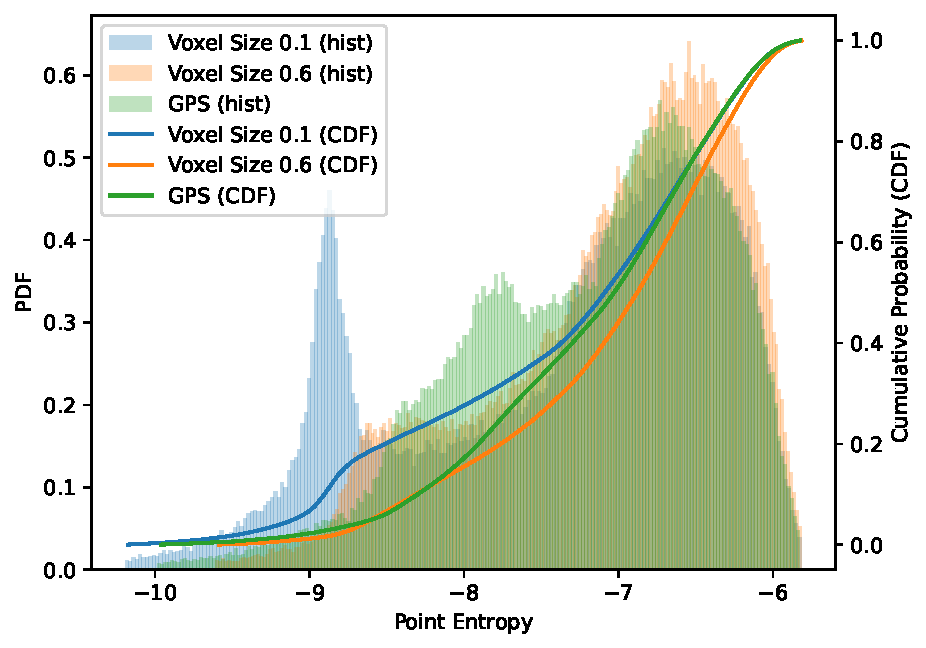
\includegraphics[width=0.45\linewidth]{images/voxel-size-entropy.pdf}
    }
    \hspace{1pt}
    \subcaptionbox{Visual comparison. }{
        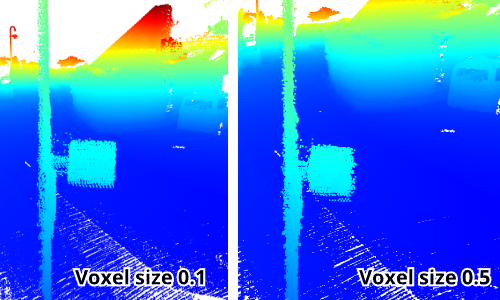
\includegraphics[width=0.47\linewidth]{images/voxel-size-comp.png}
    }
    \caption[Voxel size effect on map quality]{Voxel size effect on map quality.}
    \label{fig:voxel-size-mapping}
\end{figure}



% \begin{figure}[h]
%     \centering
%     \subcaptionbox{Translation corrections.}{
%         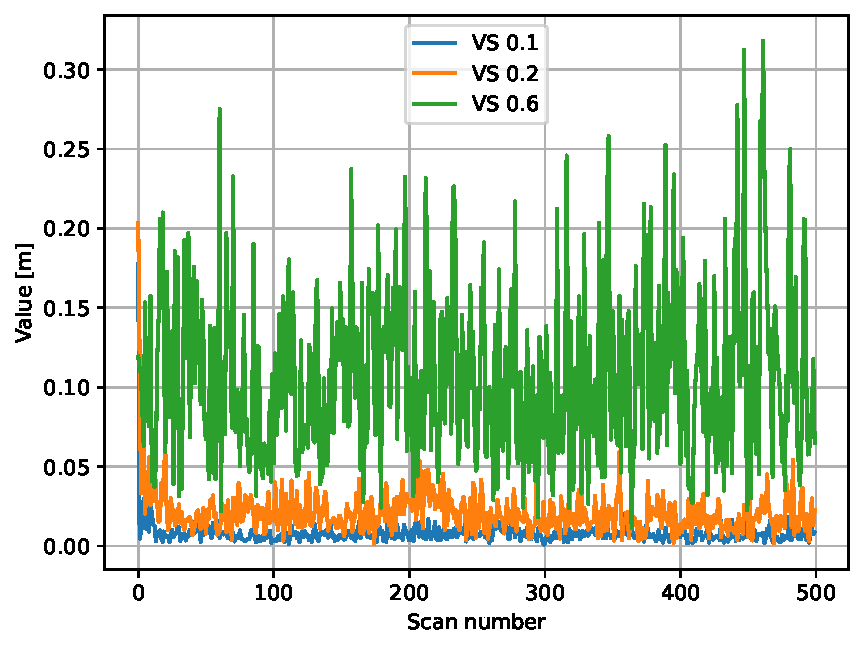
\includegraphics[width=0.46\linewidth]{images/gicp_corrections_trans.pdf}
%     }
%     \hspace{1pt}
%     \subcaptionbox{Rotation corrections.}{
%         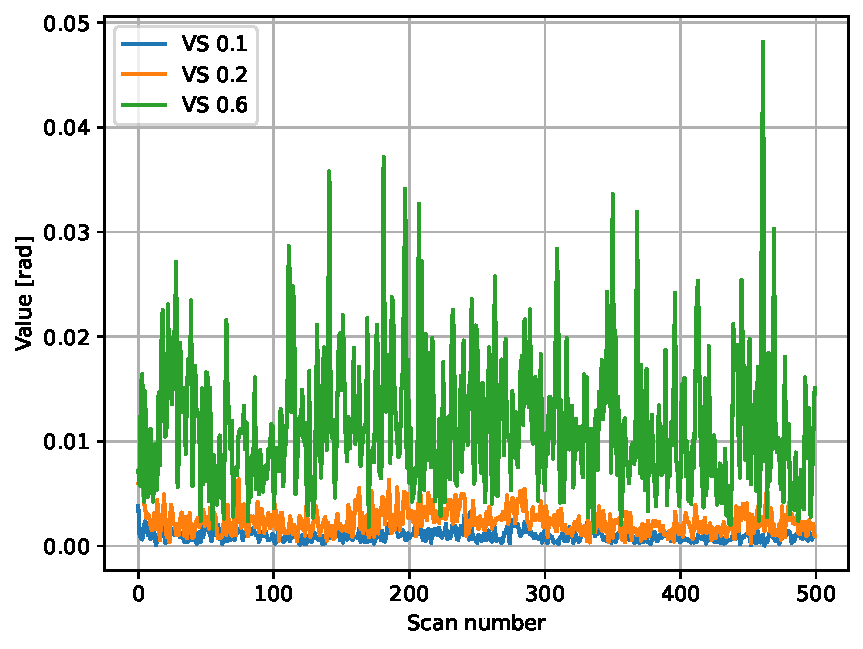
\includegraphics[width=0.45\linewidth]{images/gicp_corrections_rot.pdf}
%     }
%     \caption[]{
%     }
%     \label{fig:gicp-corrections}
% \end{figure}

\subsection{Local map size}
%% how do the results change, depending on the number of previous scans stored

Next, we observe the behavior of the algorithm in relation to the size of the local map, \ie the number of previous scans that the registration is performed against. Given the high frequency and operational range of the sensor, consecutive scans have large overlapping areas which represent useful cues for point cloud alignment. This is proven by the low odometry errors obtained for map size $\geq 5$ in Table~\ref{tab:map_sizes}. When larger maps are used, the computational time increases, without significant improvements for trajectory estimation.


\begin{table}[h]
    \centering
    \begin{tabular}{c|cccccccc}
        \hline
        \textbf{Map}  & \textbf{Median}   & \textbf{ATE}    & \textbf{ATE}  & \textbf{Final } & \textbf{Final} & \textbf{Avg.} & \textbf{Avg.}   & \textbf{Avg.}  \\
        \textbf{Size} & \textbf{Duration} & \textbf{Trans.} & \textbf{Rot.} & \textbf{Error}  & \textbf{Error} & \textbf{RMSE} & \textbf{Corr.}  & \textbf{Corr.} \\
                      &                   & \textbf{}       & \textbf{}     & \textbf{Trans.} & \textbf{Rot.}  & \textbf{}     & \textbf{Trans.} & \textbf{Rot.}  \\
        \hline \hline
        1             & 0.2349            & 5.0058          & 0.1564        & 10.2891         & 0.2603         & 0.0940        & 0.0366          & 0.0021         \\
        2             & 0.2308            & 4.3812          & 0.1355        & 9.1949          & 0.2318         & 0.0818        & 0.0171          & 0.0016         \\
        5             & 0.2632            & 1.8325          & 0.0458        & 3.6849          & 0.0734         & 0.0615        & 0.0094          & 0.0011         \\
        10            & 0.2962            & 1.2814          & 0.0294        & 2.5337          & 0.0467         & 0.0555        & 0.0080          & 0.0010         \\
        15            & 0.3242            & 1.1645          & 0.0263        & 2.2848          & 0.0415         & 0.0540        & 0.0076          & 0.0010         \\
        25            & 0.3984            & 1.1040          & 0.0245        & 2.1504          & 0.0384         & 0.0531        & 0.0079          & 0.0011         \\
        \hline
    \end{tabular}
    \caption{Metrics for varying map sizes.}
    \label{tab:map_sizes}
\end{table}

\subsection{Registration strategy}
%% how do the results change, depending on whether we use GICP or not

We also assess the influence of the Generalized ICP registration step. During the experimental phase, we observed that this has a very positive effect on accurately matching the ground plane, and this is confirmed by the metrics in Table~\ref{tab:gicp_variations}. For a more thorough analysis, we show the results corresponding to several distance threshold values, and compare against the case where only point-to-point ICP is used. The no-GICP version leads to higher trajectory errors overall, but we note that the Z component (elevation) has the highest contribution to this error. The XY error is smaller when GICP is not used \reffigbr{gicp-result-xy}, but the Z error is almost doubled \reffigbr{gicp-z-error}. In terms of map quality, using GICP clearly helps reduce point entropies and point-to-plane errors, so the surfaces of the output map capture more details, but additional constraints (\ie GPS) will help prevent drifts.

\begin{table}[h]
    \centering
    \begin{tabular}{c|cccccccc}
        \hline
        \textbf{GICP}    & \textbf{Median}   & \textbf{ATE}    & \textbf{ATE}  & \textbf{Final } & \textbf{Final} & \textbf{Avg.} & \textbf{Avg.}   & \textbf{Avg.}  \\
        \textbf{Dist.}   & \textbf{Duration} & \textbf{Trans.} & \textbf{Rot.} & \textbf{Error}  & \textbf{Error} & \textbf{RMSE} & \textbf{Corr.}  & \textbf{Corr.} \\
        \textbf{Thresh.} &                   & \textbf{}       & \textbf{}     & \textbf{Trans.} & \textbf{Rot.}  & \textbf{}     & \textbf{Trans.} & \textbf{Rot.}  \\
        \hline \hline
        -                & 0.2111            & 1.8036          & 0.0371        & 2.8009          & 0.0571         & 0.0601        & -               & -              \\
        0.1              & 0.2949            & 1.1686          & 0.0275        & 1.5486          & 0.0357         & 0.0457        & 0.0070          & 0.0009         \\
        0.2              & 0.3020            & 1.1167          & 0.0280        & 1.4442          & 0.0340         & 0.0520        & 0.0070          & 0.0009         \\
        0.5              & 0.2860            & 1.1958          & 0.0326        & 1.4858          & 0.0390         & 0.0599        & 0.0073          & 0.0010         \\
        \hline
    \end{tabular}
    \caption{Metrics for GICP variations.}
    \label{tab:gicp_variations}
\end{table}

\begin{figure}[h]
    \centering
    \subcaptionbox{Trajectory end point location. \label{fig:gicp-result-xy}}{
        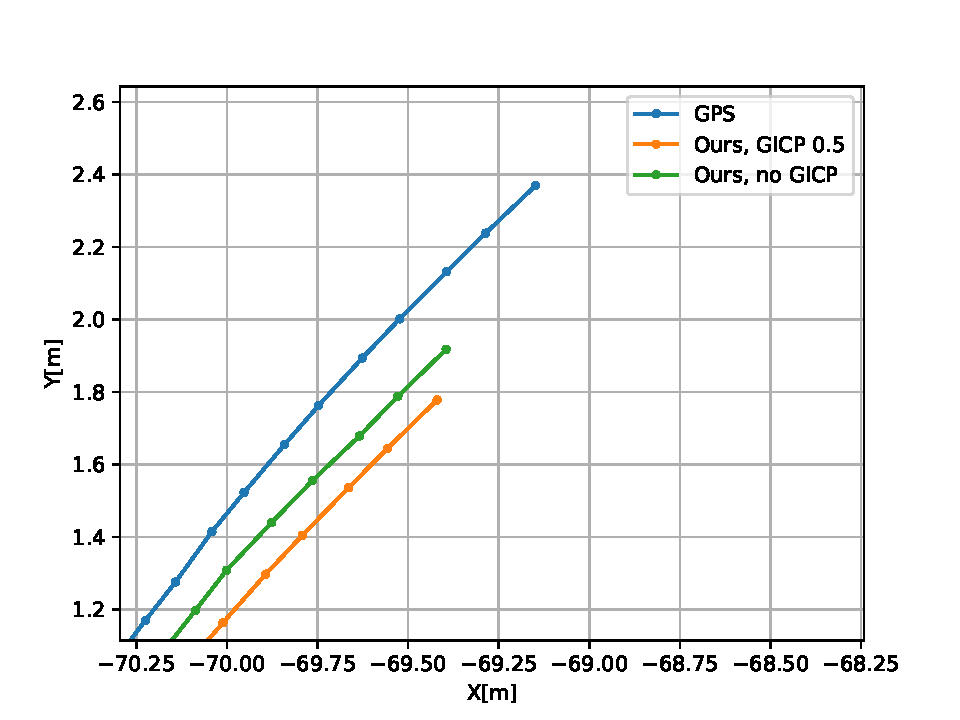
\includegraphics[width=0.47\linewidth]{images/gicp-result-xy.pdf}
    }
    \hspace{1pt}
    \subcaptionbox{Z error evolution.\label{fig:gicp-z-error}}{
        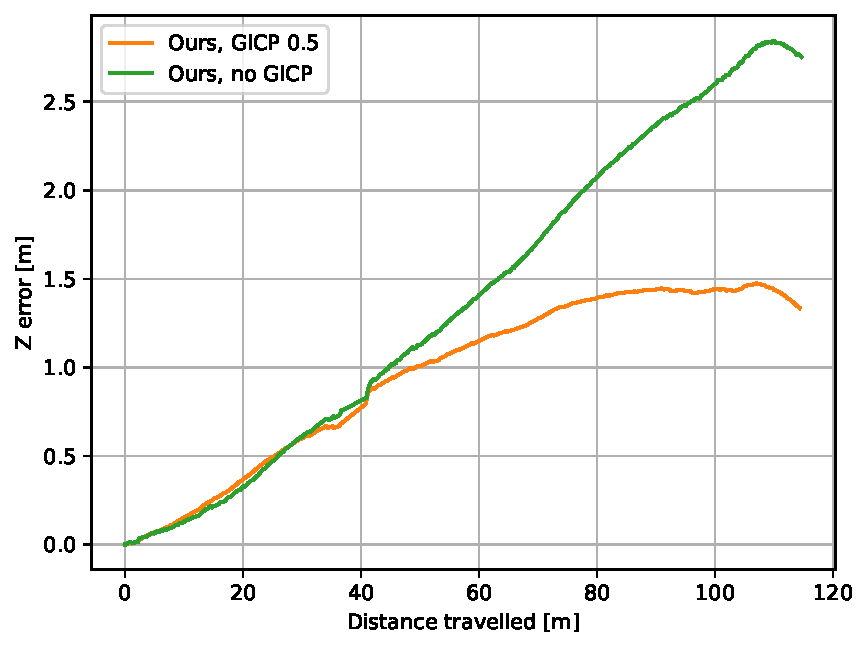
\includegraphics[width=0.44\linewidth]{images/gicp-z-error.pdf}
    }
    \caption[Trajectory evaluation with and without GICP]{Trajectory evaluation with and without GICP.}
    \label{fig:gicp-traj-result}
\end{figure}

\begin{figure}[h]
    \centering
    \subcaptionbox{Distribution of point entropies.}{
        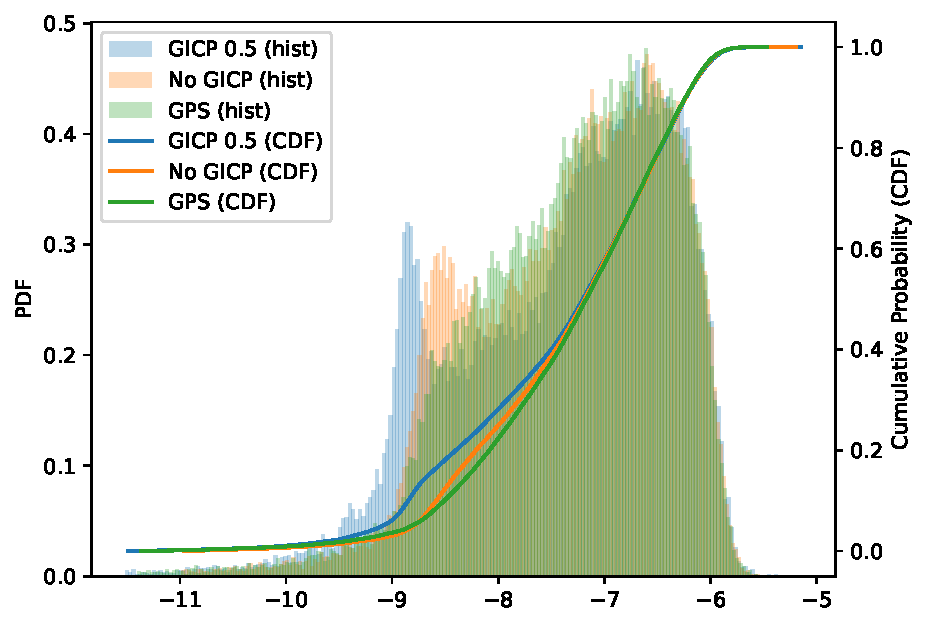
\includegraphics[width=0.46\linewidth]{images/gicp-map-entropy.pdf}
    }
    \hspace{1pt}
    \subcaptionbox{Point-to-plane errors (first 20 scans)}{
        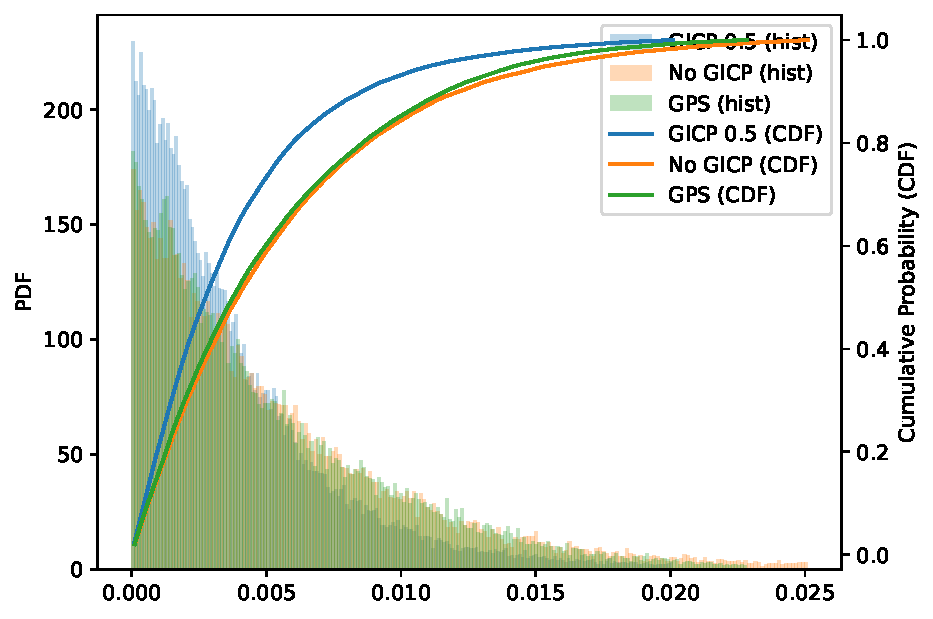
\includegraphics[width=0.45\linewidth]{images/gicp-p2plane.pdf}
    }
    % \subcaptionbox{Observing the Z difference in CloudCompare. Yellow - without GICP, white - with GICP.}{
    %     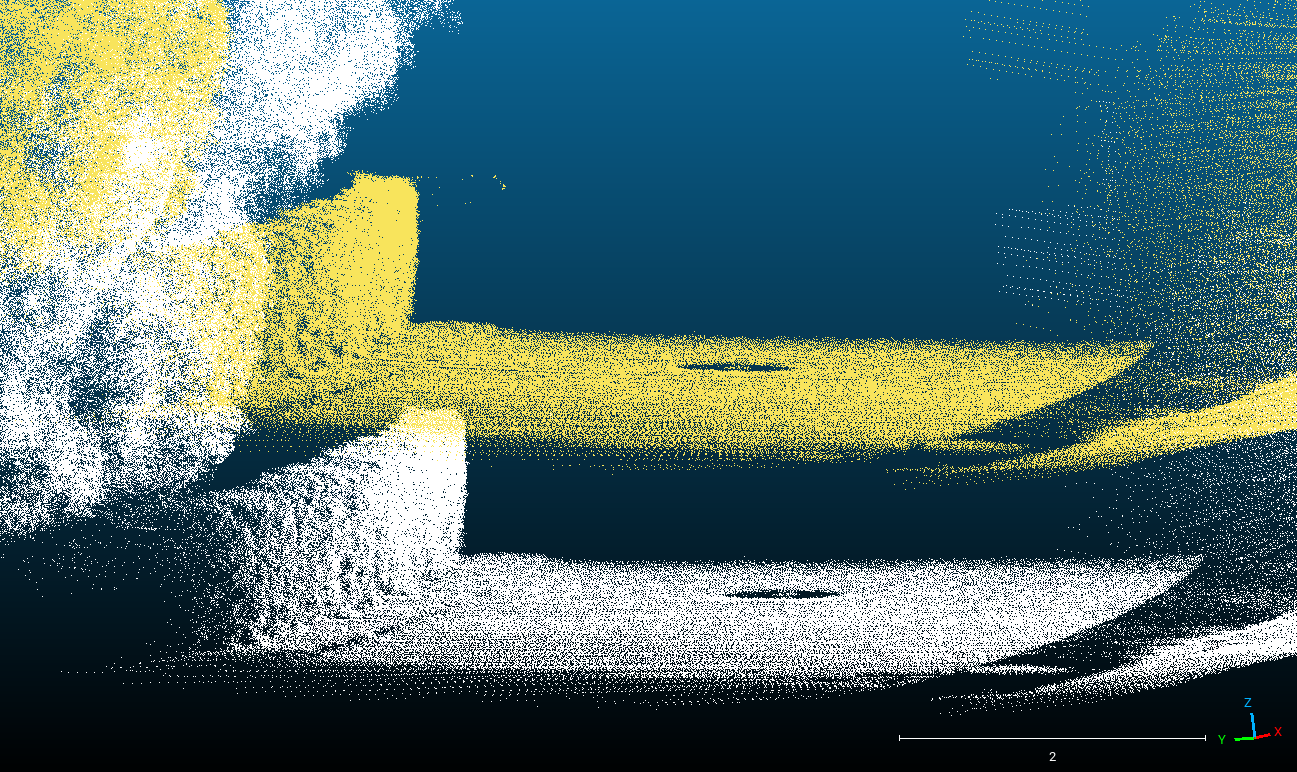
\includegraphics[width=0.45\linewidth]{images/gicp-z-error-view.png}
    % }
    \caption[Map evaluation with and without GICP]{Map evaluation with and without GICP.}
    \label{fig:gicp-map-result}
\end{figure}


\section{Odometry evaluation}

The first odometry evaluation we perform is on the trajectory recorded with the \mbox{SDX-Compact} system, depicted in \reffig{odom-traj}. We do not use the GPS data during execution, but treat it as ground truth to obtain the trajectory error metrics in Table~\ref{tab:custom-traj-results}. Because we consider scan timestamps during motion prediction, we are able to handle large ``jumps'' in the scan sequence \reffigbr{odom-jumps}, something that other methods struggle with. However, elevation estimation is still an issue, as seen in \reffig{z-dif-traj}.

\begin{figure}[h]
    \centering
    \subcaptionbox{Full trajectory comparison.}{
        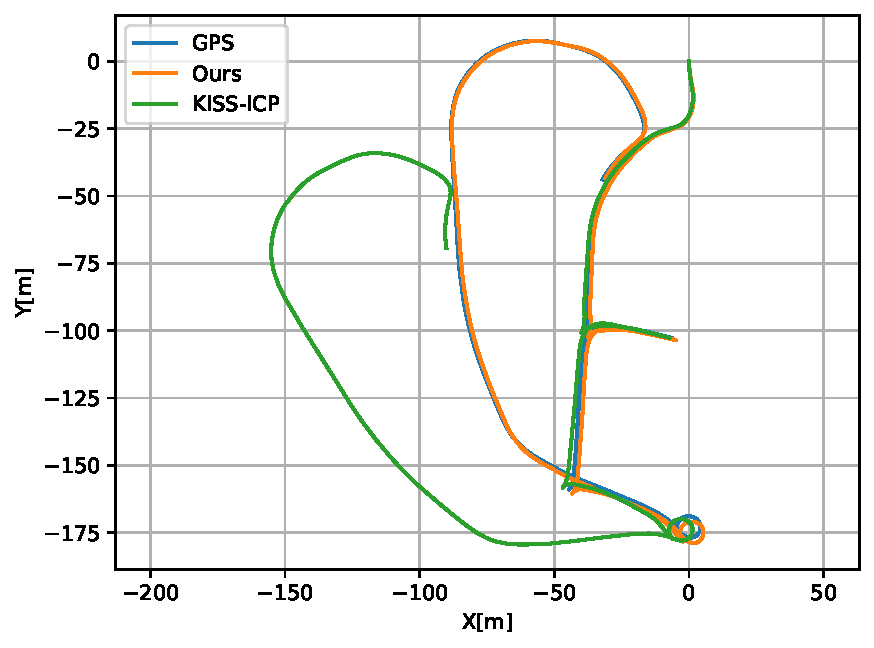
\includegraphics[width=0.445\linewidth]{images/eval_traj/traj.pdf}
    }
    \hspace{1pt}
    \subcaptionbox{A troublesome region with time jumps. \label{fig:odom-jumps}}{
        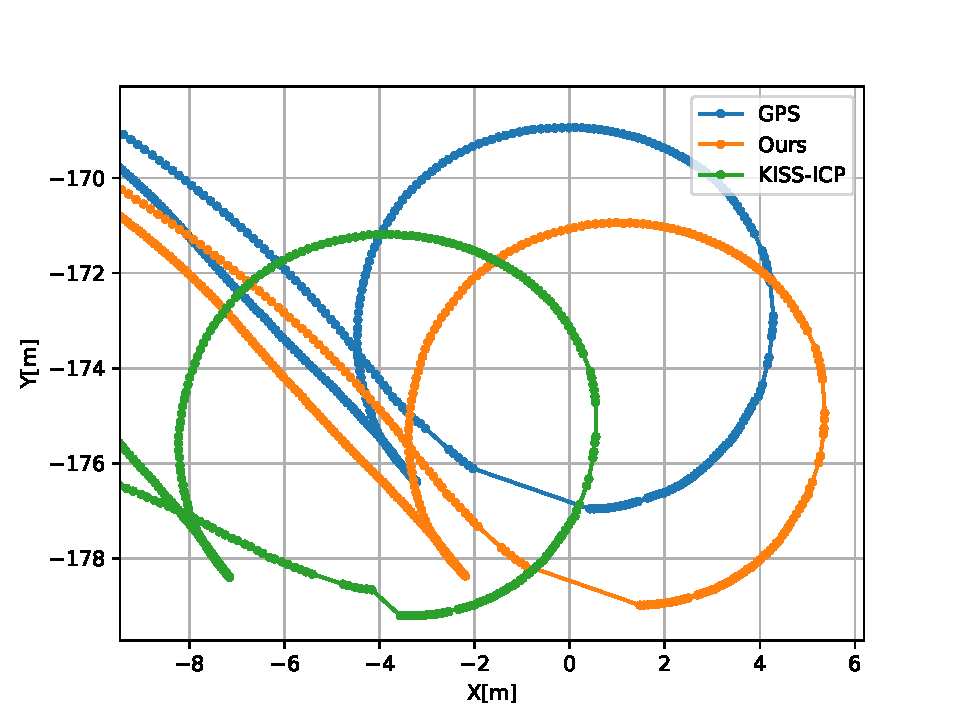
\includegraphics[width=0.485\linewidth]{images/eval_traj/loop.pdf}
    }
    \caption[Odometry evaluation on custom trajectory]{Odometry evaluation on custom trajectory: our method and KISS-ICP \cite{vizzo2023ral} against GPS data.}
    \label{fig:odom-traj}
\end{figure}

\begin{table}[h]
    \centering
    \begin{tabular}{c|cc|cc|cc|cc|cc}
        \hline
                       &                                    &                                     &                            &                             & \multicolumn{6}{c}{\textbf{Avg. RTE}}                                                                                 \\
                       & \multicolumn{2}{c|}{ \textbf{ATE}} & \multicolumn{2}{c|}{\textbf{Final}} & \multicolumn{2}{c|}{$k=1$} & \multicolumn{2}{c|}{$k=10$} & \multicolumn{2}{c}{$k=100$}                                                                                           \\
                       & \textbf{tra.}                      & \textbf{rot.}                       & \textbf{tra.}              & \textbf{rot.}               & \textbf{tra.}                         & \textbf{rot.} & \textbf{tra.} & \textbf{rot.} & \textbf{tra.} & \textbf{rot.} \\
        \hline
        \hline
        \textbf{K-ICP} & 46.879                             & 0.407                               & 65.965                     & 0.688                       & 3.72                                  & 28.89         & 1.95          & 17.31         & 3.05          & 17.49         \\
        \textbf{Ours}  & 8.232                              & 0.102                               & 1.311                      & 0.095                       & 2.81                                  & 16.67         & 1.36          & 10.88         & 1.15          & 11.28         \\
        \hline
    \end{tabular}
    \caption{Comparison with KISS-ICP \cite{vizzo2023ral} on custom trajectory. We report RTE~(\%) for sub-sequences of various lengths ($k$ is the number of LiDAR scans). }
    \label{tab:custom-traj-results}
\end{table}

\begin{figure}[h]
    \centering
    \subcaptionbox{XY errors. The KISS-ICP method diverges after a jump in the sequence.}{
        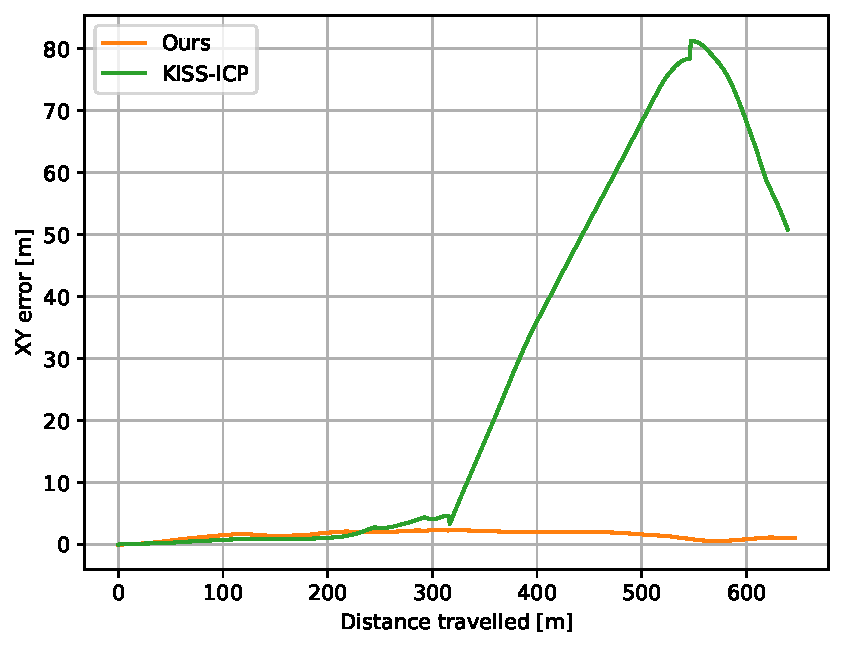
\includegraphics[width=0.455\linewidth]{images/eval_traj/xy_errors.pdf}
    }
    \hspace{1pt}
    \subcaptionbox{Z values. Both methods struggle to correctly estimate the Z component of the location. \label{fig:z-dif-traj}}{
        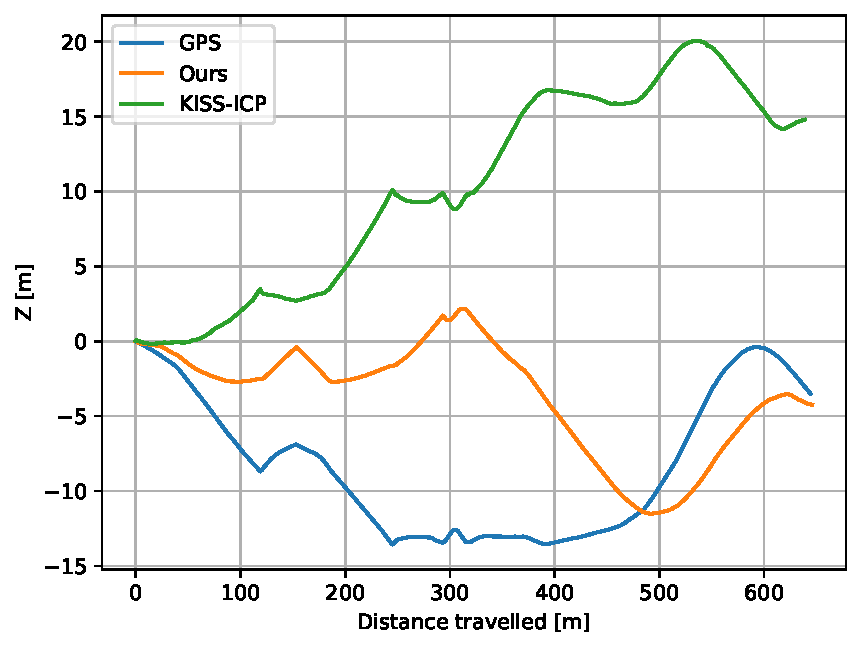
\includegraphics[width=0.475\linewidth]{images/eval_traj/Zs.pdf}
    }
    \caption[Position analysis on custom trajectory]{Position analysis on custom trajectory. }
    \label{fig:xyz-traj}
\end{figure}
We also evaluate on the sequences of the KITTI dataset \cite{geiger2013vision} which include ground-truth pose values from a GPS + IMU sensor system. This is a popular benchmark for urban SLAM problems, and it represents an interesting challenge for our solution because it uses a different LiDAR sensor (Velodyne HDL-64E), the environment is different, and moving vehicles are present. To operate on this dataset, we adjust the solution as follows:
\begin{compactitem}
    \item Discard LiDAR points that are farther than 50m or closer than 1m, to avoid high distortion and points belonging to the sensor rig

    \item Use a larger base voxel size: as the scanned environment is larger, we use a default voxel size of 0.2m instead of 0.1m
\end{compactitem}
The results of this evaluation are presented in Table~\ref{tab:odom-kitti}.

\begin{table}[h]
    \centering
    % \begin{tabular}{c|c|ccc|cc|cccc}
    %     \hline
    %                   &                 &                                   &                                     &                            &                             &               & \textbf{}     & \multicolumn{2}{c}{\textbf{Avg. RTE}} &                               \\
    %     \textbf{Seq.} & \textbf{}       & \multicolumn{3}{c|}{\textbf{ATE}} & \multicolumn{2}{c|}{\textbf{Final}} & \multicolumn{2}{c|}{$k=1$} & \multicolumn{2}{c}{$k=100$}                                                                                                         \\
    %     \textbf{no.}  & \textbf{Length} & \textbf{XY}                       & \textbf{tra.}                       & \textbf{rot.}              & \textbf{tra.}               & \textbf{rot.} & \textbf{tra.} & \multicolumn{1}{c|}{\textbf{rot.}}    & \textbf{tra.} & \textbf{rot.} \\ \hline \hline
    %     00            & 3723.24         & 7.29                              & 16.28                               & 0.07                       & 11.58                       & 0.06          & 3.0           & 21.01                                 & 1.19          & 11.71         \\
    %     01            & 2453.26         & 24.53                             & 190.1                               & 0.21                       & 291.51                      & 0.3           & 1.6           & 37.07                                 & 1.95          & 55.96         \\
    %     02            & 5067.02         & 22.2                              & 50.39                               & 0.13                       & 99.53                       & 0.22          & 2.17          & 19.95                                 & 1.2           & 12.24         \\
    %     03            & 560.85          & 2.92                              & 8.84                                & 0.05                       & 18.15                       & 0.08          & 2.87          & 18.26                                 & 0.83          & 7.69          \\
    %     04            & 393.65          & 0.72                              & 4.98                                & 0.03                       & 11.76                       & 0.06          & 1.3           & 33.69                                 & 1.15          & 271.49        \\
    %     05            & 2205.2          & 4.62                              & 6.92                                & 0.04                       & 13.79                       & 0.07          & 4.4           & 22.89                                 & 0.89          & 21.12         \\ \hline
    % \end{tabular}
    \begin{tabular}{c|c|ccc|ccc|ccc}
        \hline
                      &                 & \multicolumn{3}{c|}{\textbf{ATE}} & \multicolumn{3}{c|}{\textbf{Final}} & \multicolumn{3}{c}{\textbf{Avg. RTE} (100m)}                                                                                             \\
        \textbf{Seq.} & \textbf{Length} & \textbf{XY}                       & \textbf{Tra.}                       & \textbf{Rot.}                                & \textbf{XY} & \textbf{Tra.} & \textbf{Rot.} & \textbf{XY} & \textbf{Tra.} & \textbf{Rot.} \\
        \hline \hline
        00            & 3723.24         & 7.29                              & 16.28                               & 0.07                                         & 10.59       & 11.58         & 0.06          & 0.81        & 1.23          & 12.88         \\
        01            & 2453.26         & 24.53                             & 190.1                               & 0.21                                         & 39.9        & 291.51        & 0.3           & 0.98        & 1.31          & 45.7          \\
        02            & 5067.02         & 22.2                              & 50.39                               & 0.13                                         & 49.72       & 99.53         & 0.22          & 0.7         & 1.22          & 11.99         \\
        03            & 560.85          & 2.92                              & 8.84                                & 0.05                                         & 6.35        & 18.15         & 0.08          & 0.57        & 0.67          & 7.69          \\
        04            & 393.65          & 0.72                              & 4.98                                & 0.03                                         & 1.16        & 11.76         & 0.06          & 0.39        & 0.89          & 125.81        \\
        05            & 2205.2          & 4.62                              & 6.92                                & 0.04                                         & 9.2         & 13.79         & 0.07          & 0.5         & 1.02          & 20.44         \\
        06            & 1232.69         & 2.03                              & 3.78                                & 0.03                                         & 4.88        & 8.79          & 0.05          & 0.59        & 0.91          & 54.07         \\
        07            & 694.39          & 0.5                               & 1.8                                 & 0.02                                         & 0.96        & 1.36          & 0.02          & 0.58        & 1.0           & 5.12          \\
        08            & 3222.02         & 16.73                             & 28.33                               & 0.08                                         & 20.9        & 33.15         & 0.11          & 1.04        & 1.52          & 24.66         \\
        09            & 1704.96         & 6.12                              & 14.12                               & 0.06                                         & 9.28        & 9.78          & 0.04          & 0.68        & 1.03          & 8.1           \\
        10            & 919.4           & 3.94                              & 18.8                                & 0.07                                         & 4.61        & 21.78         & 0.09          & 0.65        & 1.04          & 8.79          \\
        \hline
    \end{tabular}
    \caption{Odometry evaluation on KITTI sequences. We report the XY-only error values to emphasize localization performance. RTE values are reported in \%, averaged over all 100m sub-sequences.}
    \label{tab:odom-kitti}
\end{table}

\section{GPS-integrated evaluation}
% using noisy gps on our data

% using less gps on our data


\section{Mapping evaluation}

% \section{KITTI results}

% Things worth mentioning
% - execution time